\section{Grundglieder \skript{25ff, 202-206}}

	\subsection{statische Glieder \skript{28}}
		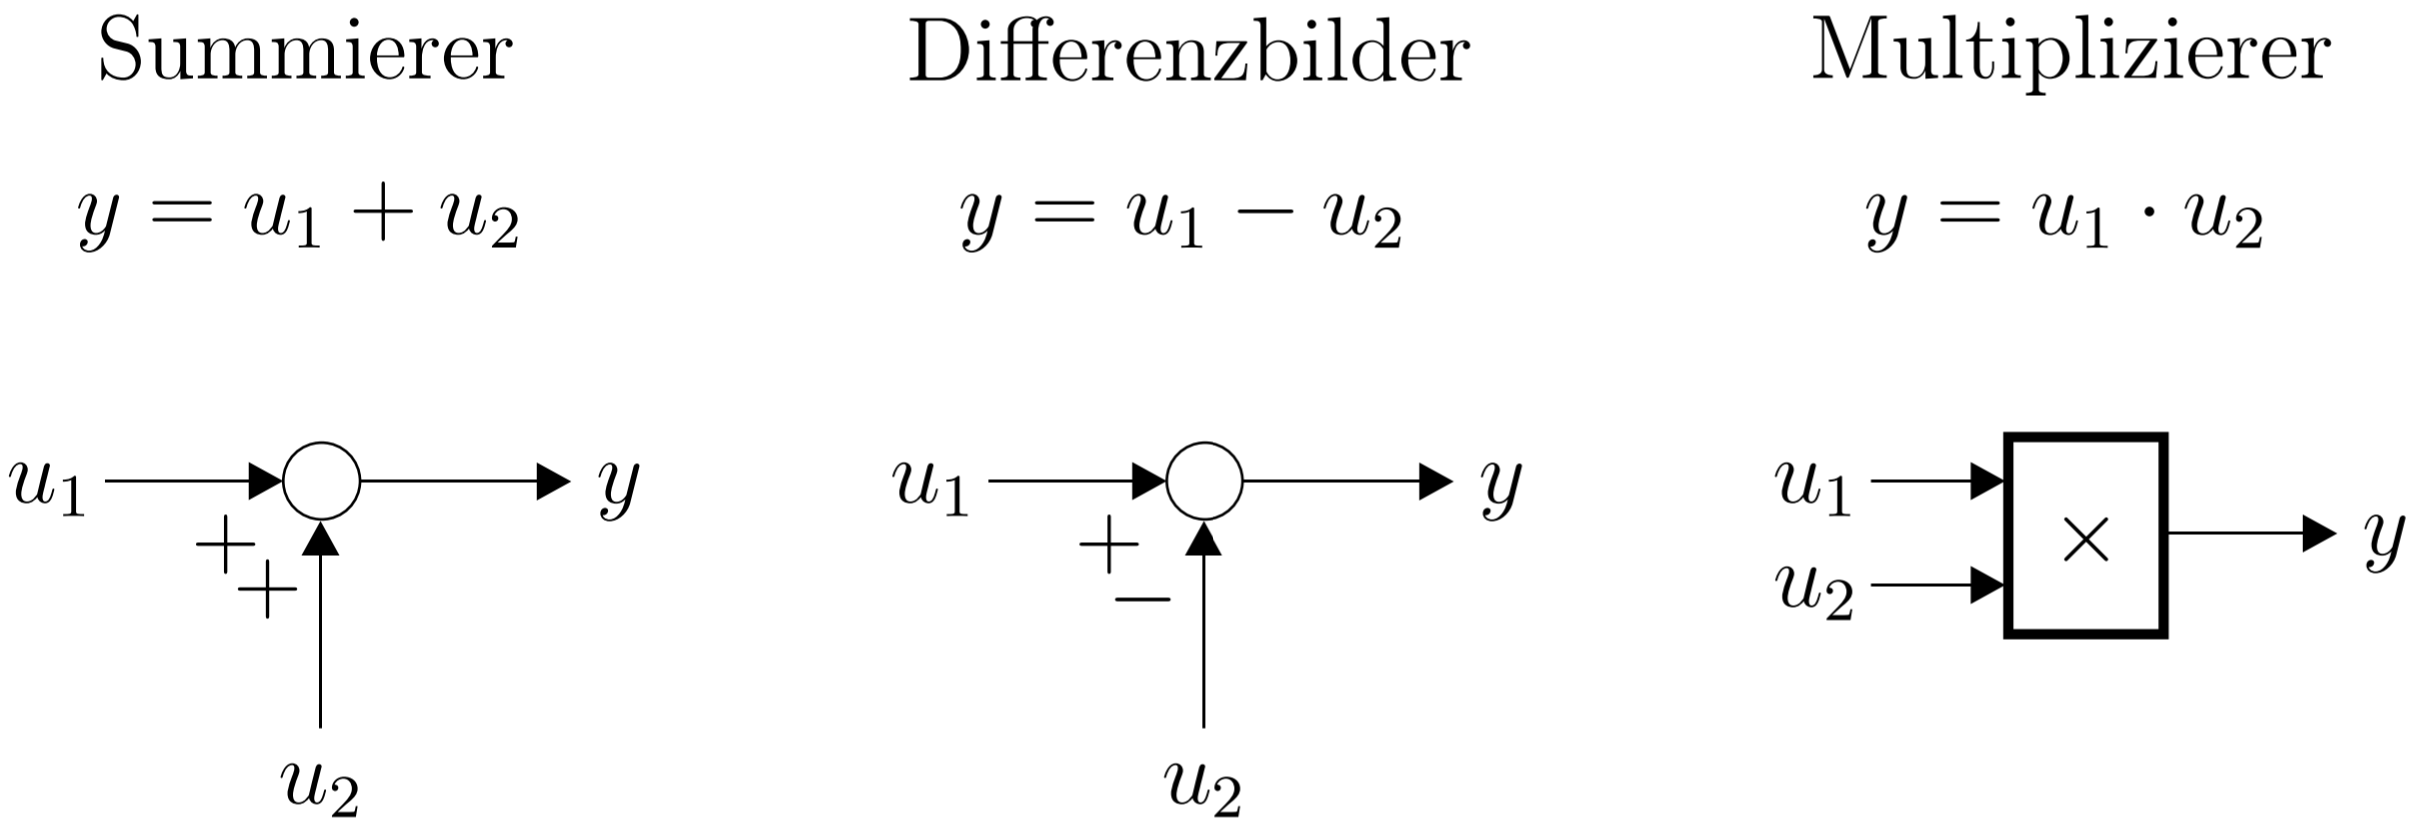
\includegraphics[width=10 cm]{./bilder/grundglieder/statischeGlieder.png} \\
		
	\subsection {Elektronische Schaltungen}
		\begin{minipage}{7cm}
			\textbf{P-Glied (nicht inv. Op-Amp)}\\
			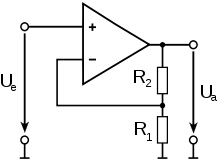
\includegraphics[height=2.5cm]{./bilder/OP-Amp.png} \\
			$K = 1 + \frac{R_2}{R_1}$
		\end{minipage}
		\begin{minipage}{6cm}
			\textbf{P-Glied (inv. Op-Amp)} \\ 
			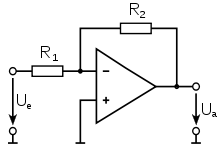
\includegraphics[height=2.5cm]{./bilder/OP-InvAmp.png} \\
			$K=-\frac{R_2}{R_1}$
		\end{minipage}
		\begin{minipage}{6cm}
			\textbf{I-Glied} \\ 
			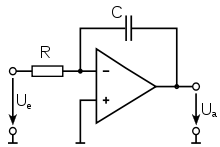
\includegraphics[height=2.5cm]{./bilder/OP-Integrator.png}\\
			$K = - \frac{1}{R \cdot C}$
		\end{minipage}  
	
	
	\subsection{dynamische Glieder \skript{25-41, 202-206}}
			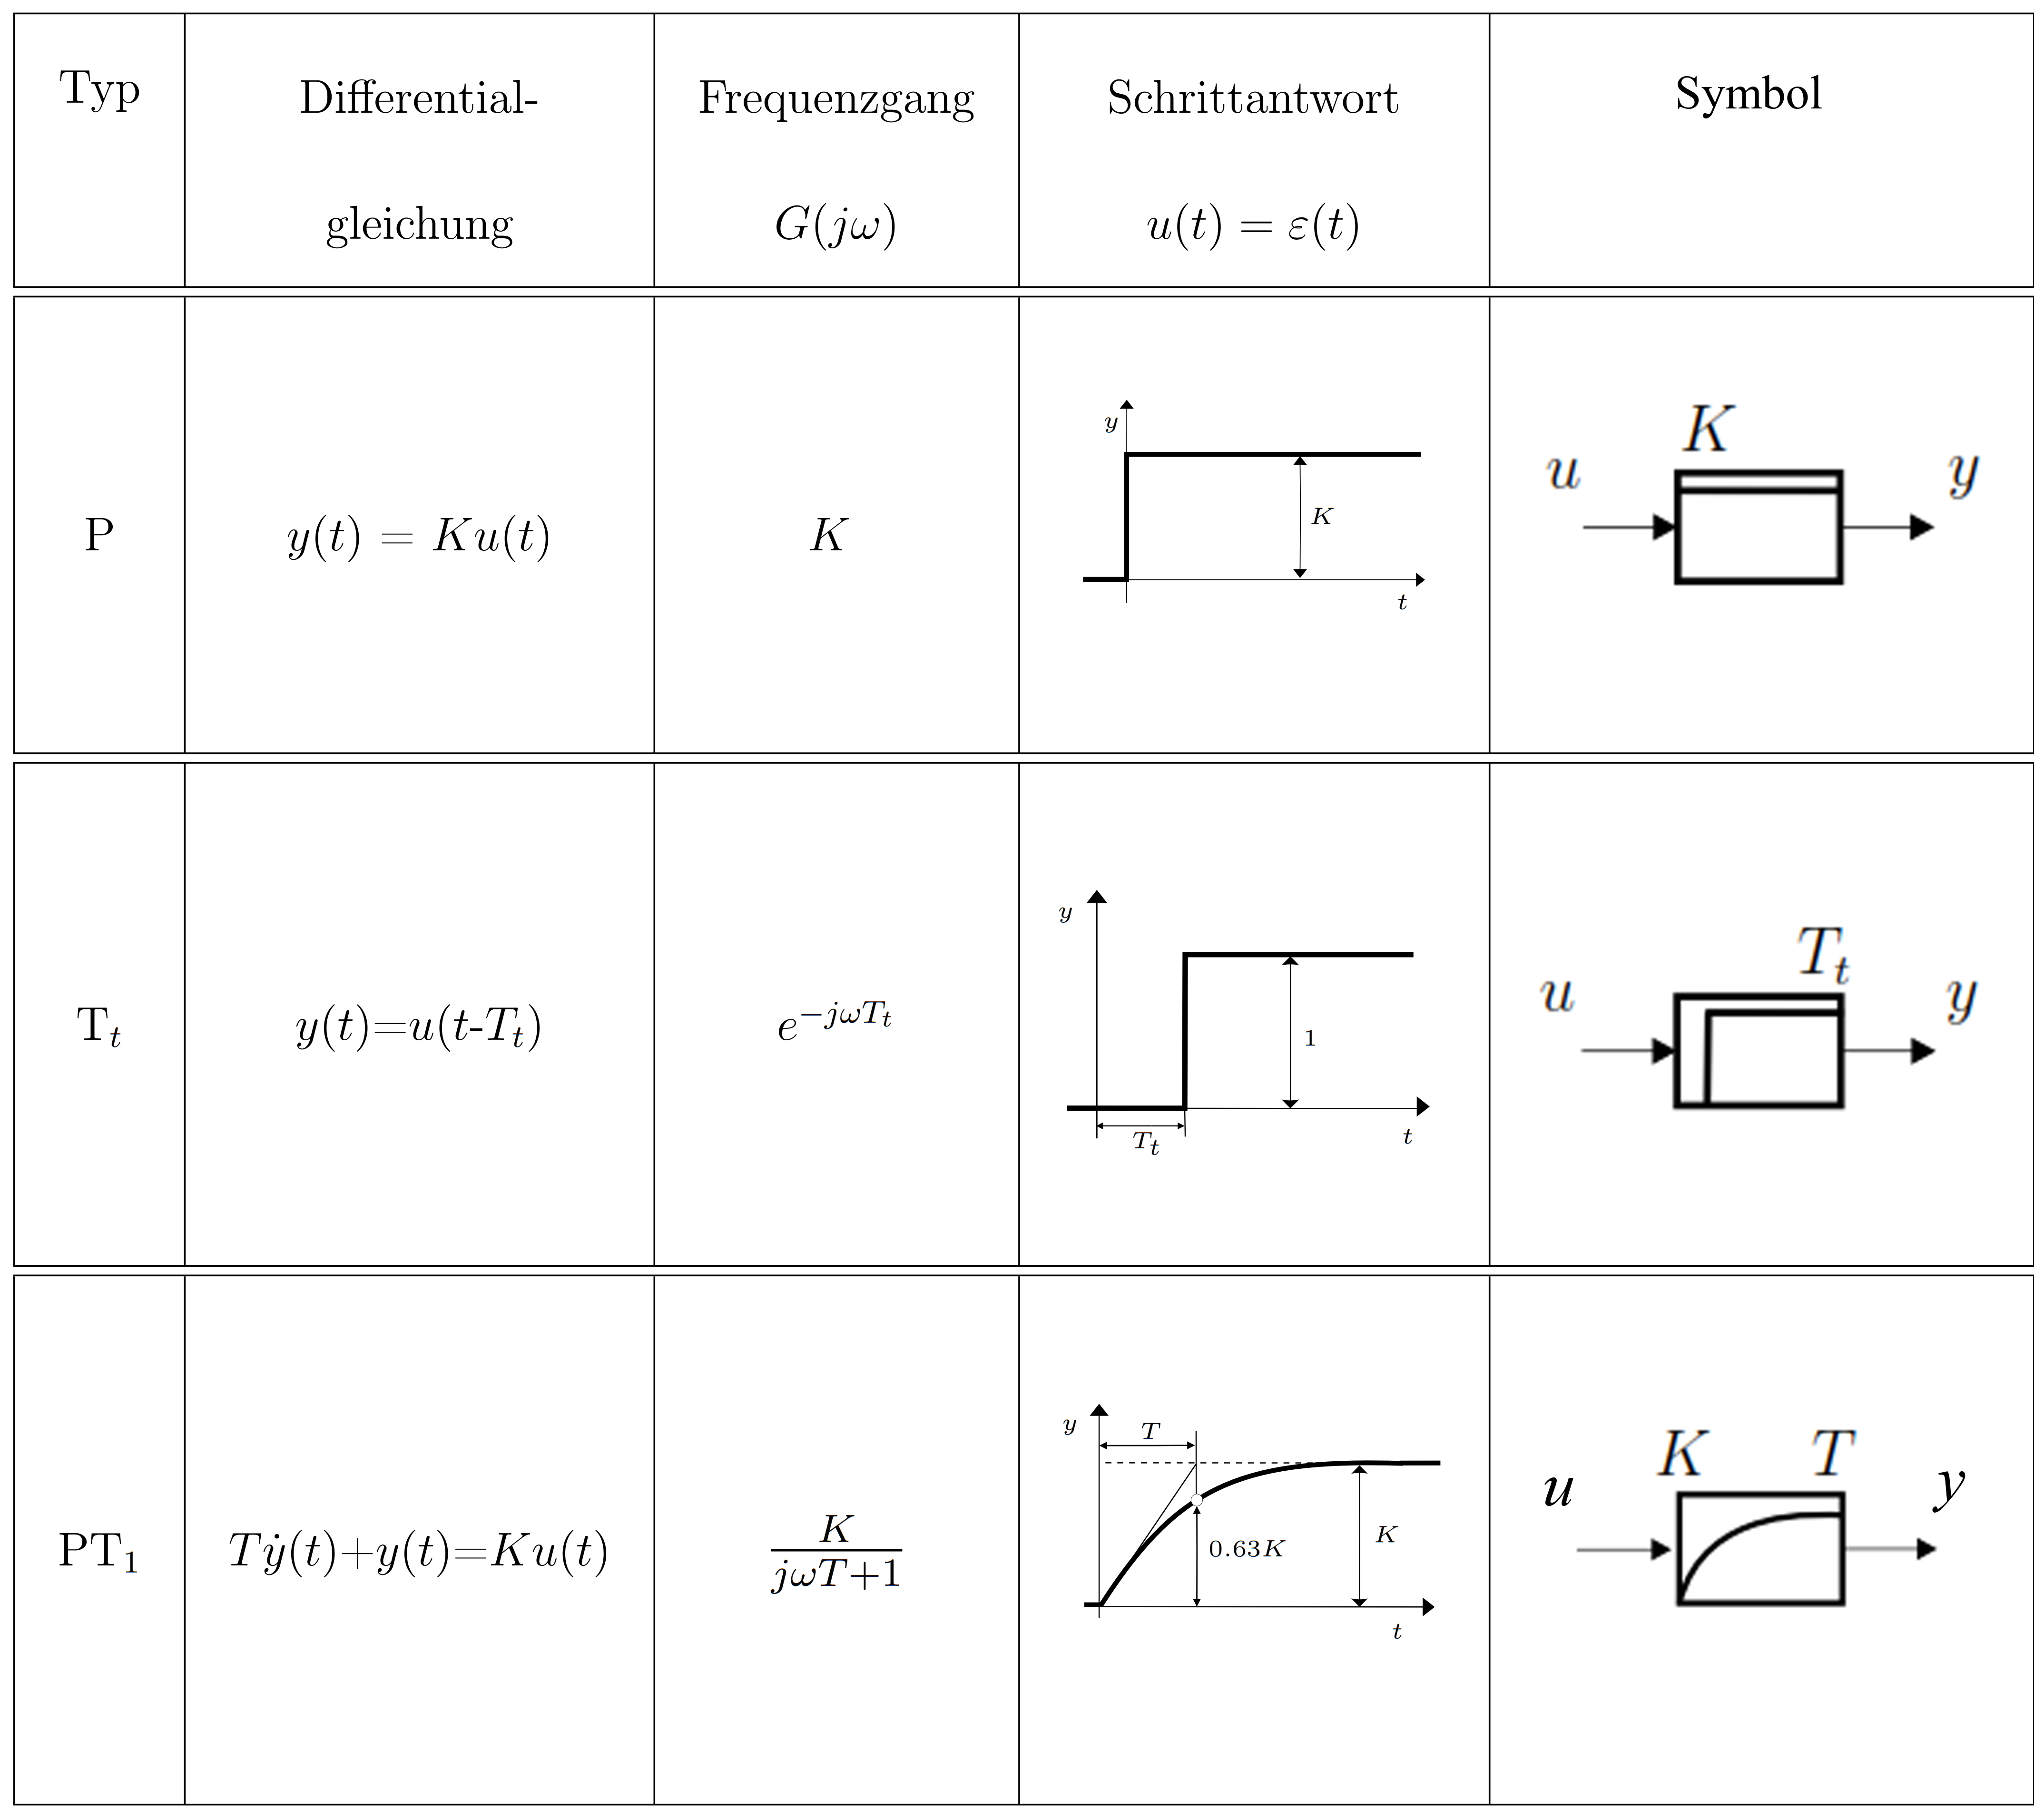
\includegraphics[width=13.5 cm]{./bilder/grundglieder/tabelle/glieder1.png} \\
			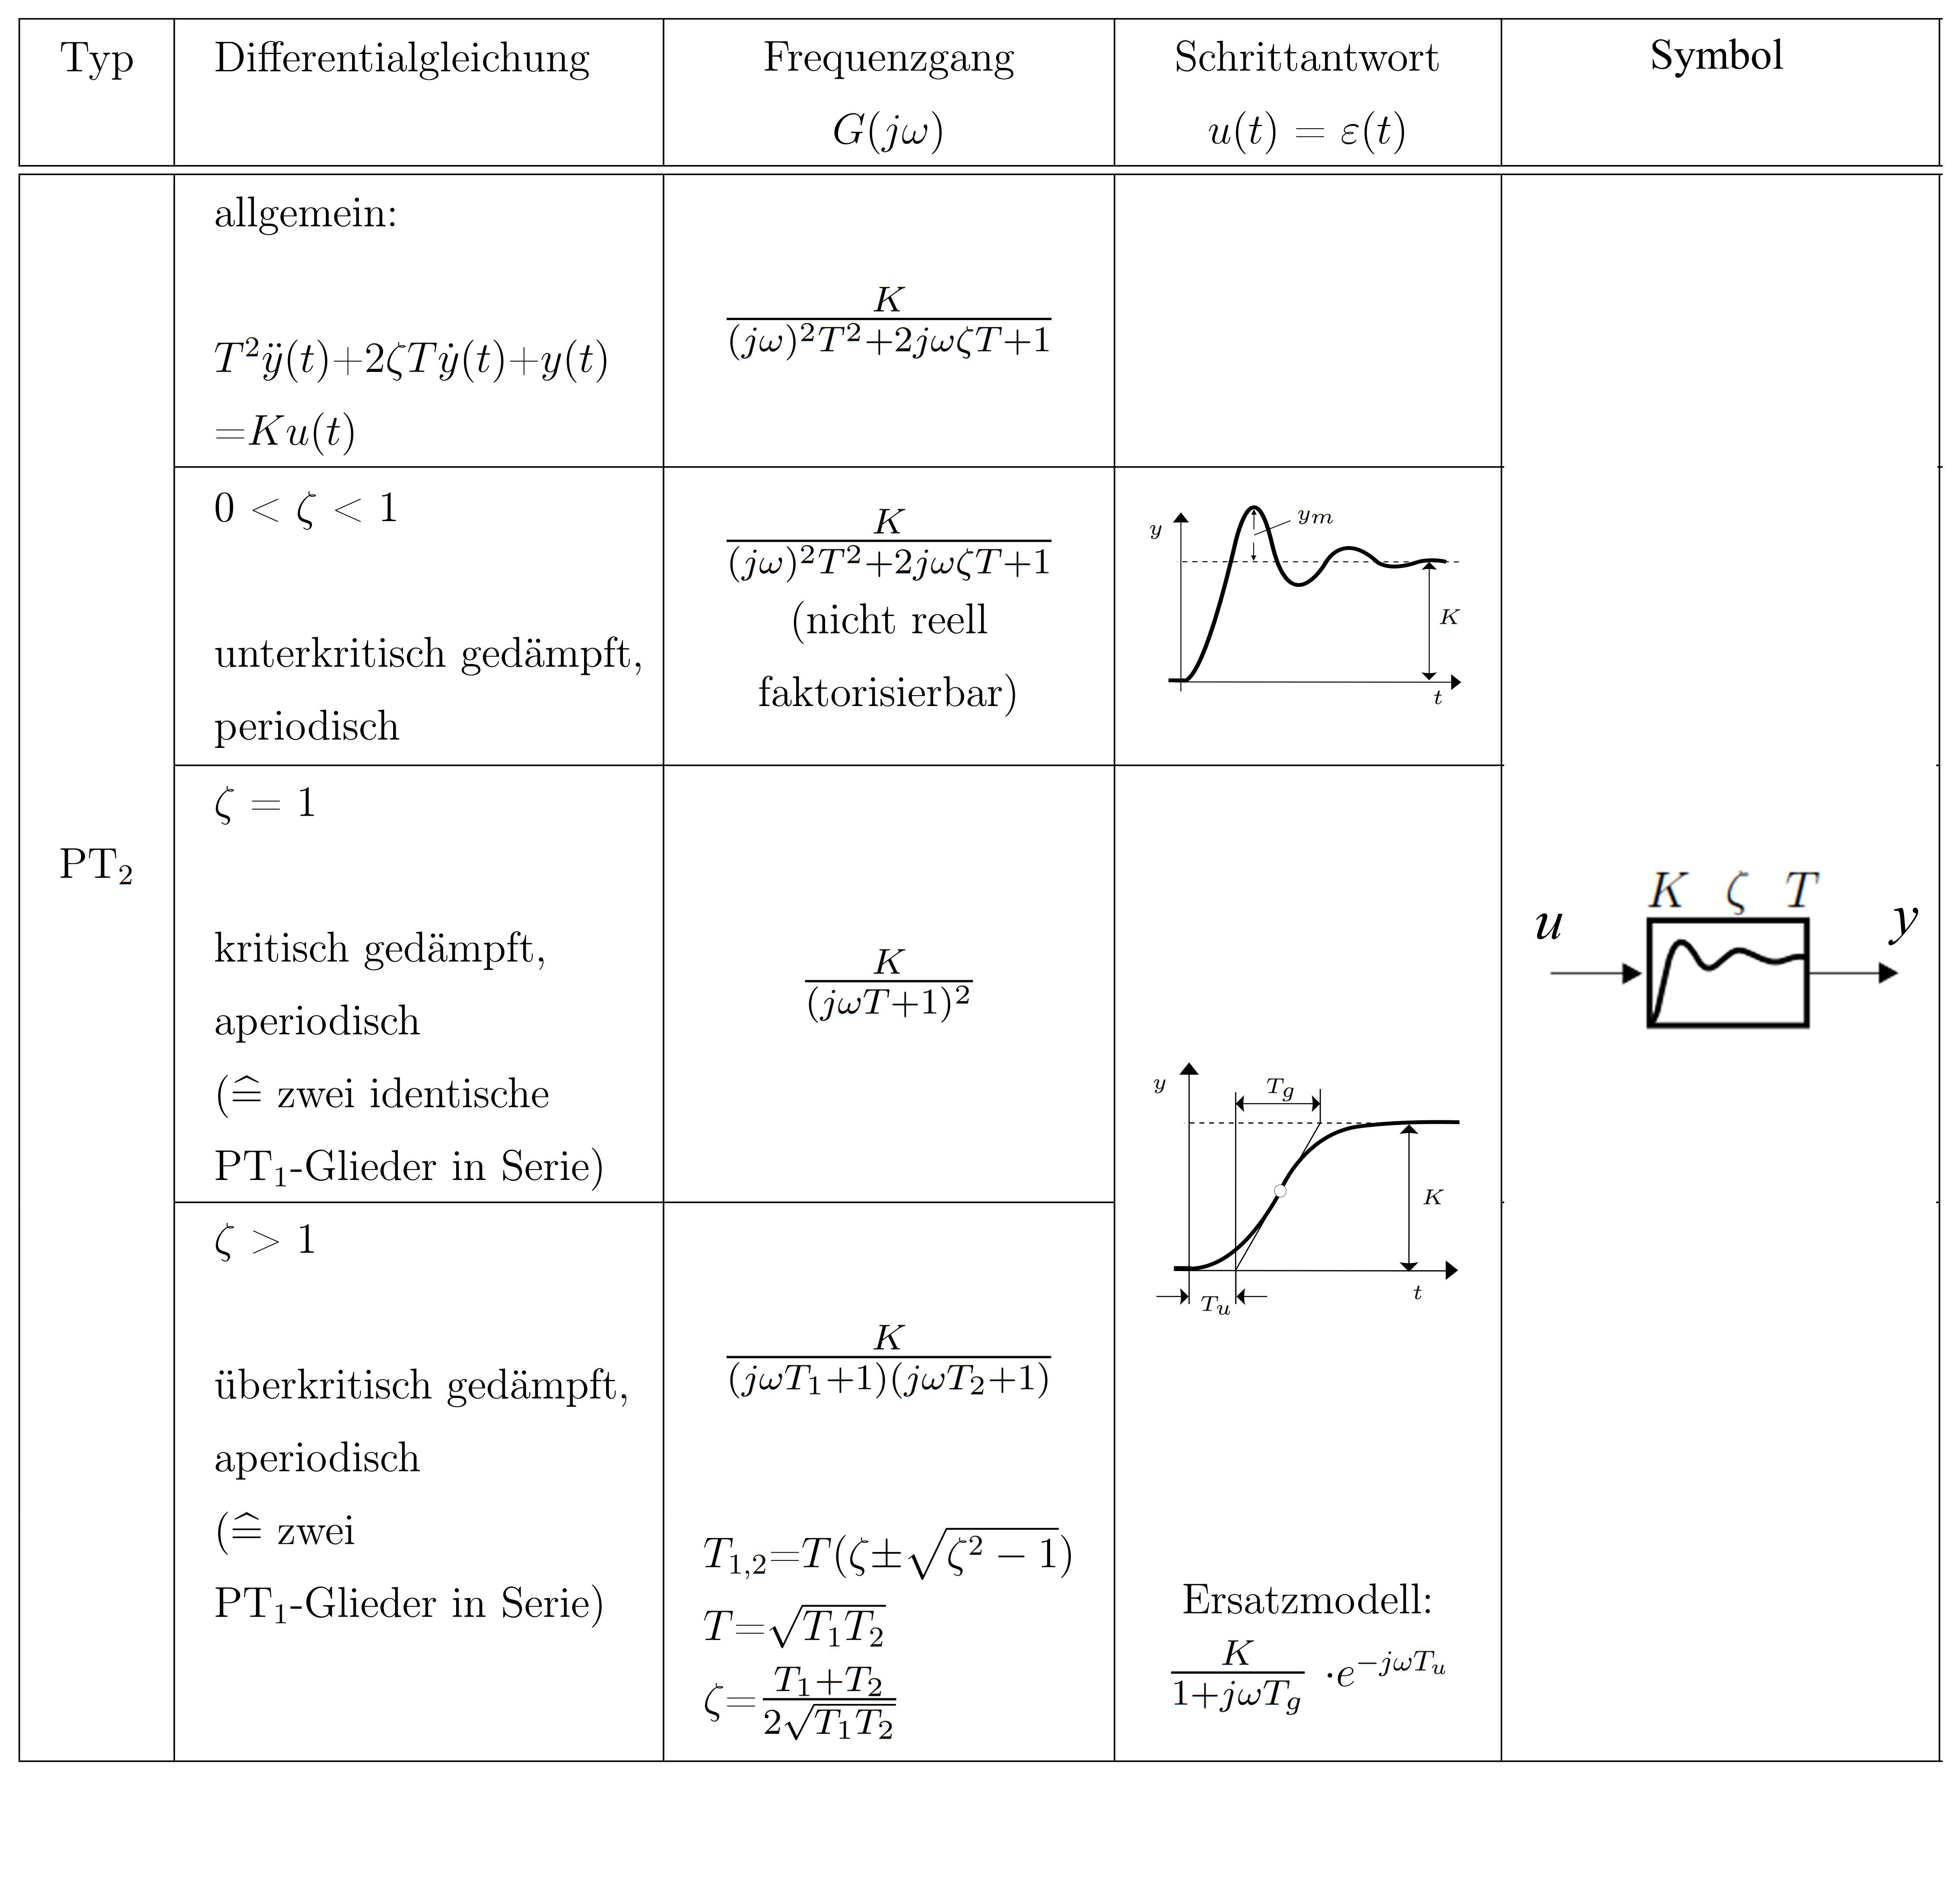
\includegraphics[width=13.5 cm]{./bilder/grundglieder/tabelle/glieder2.png} \\
			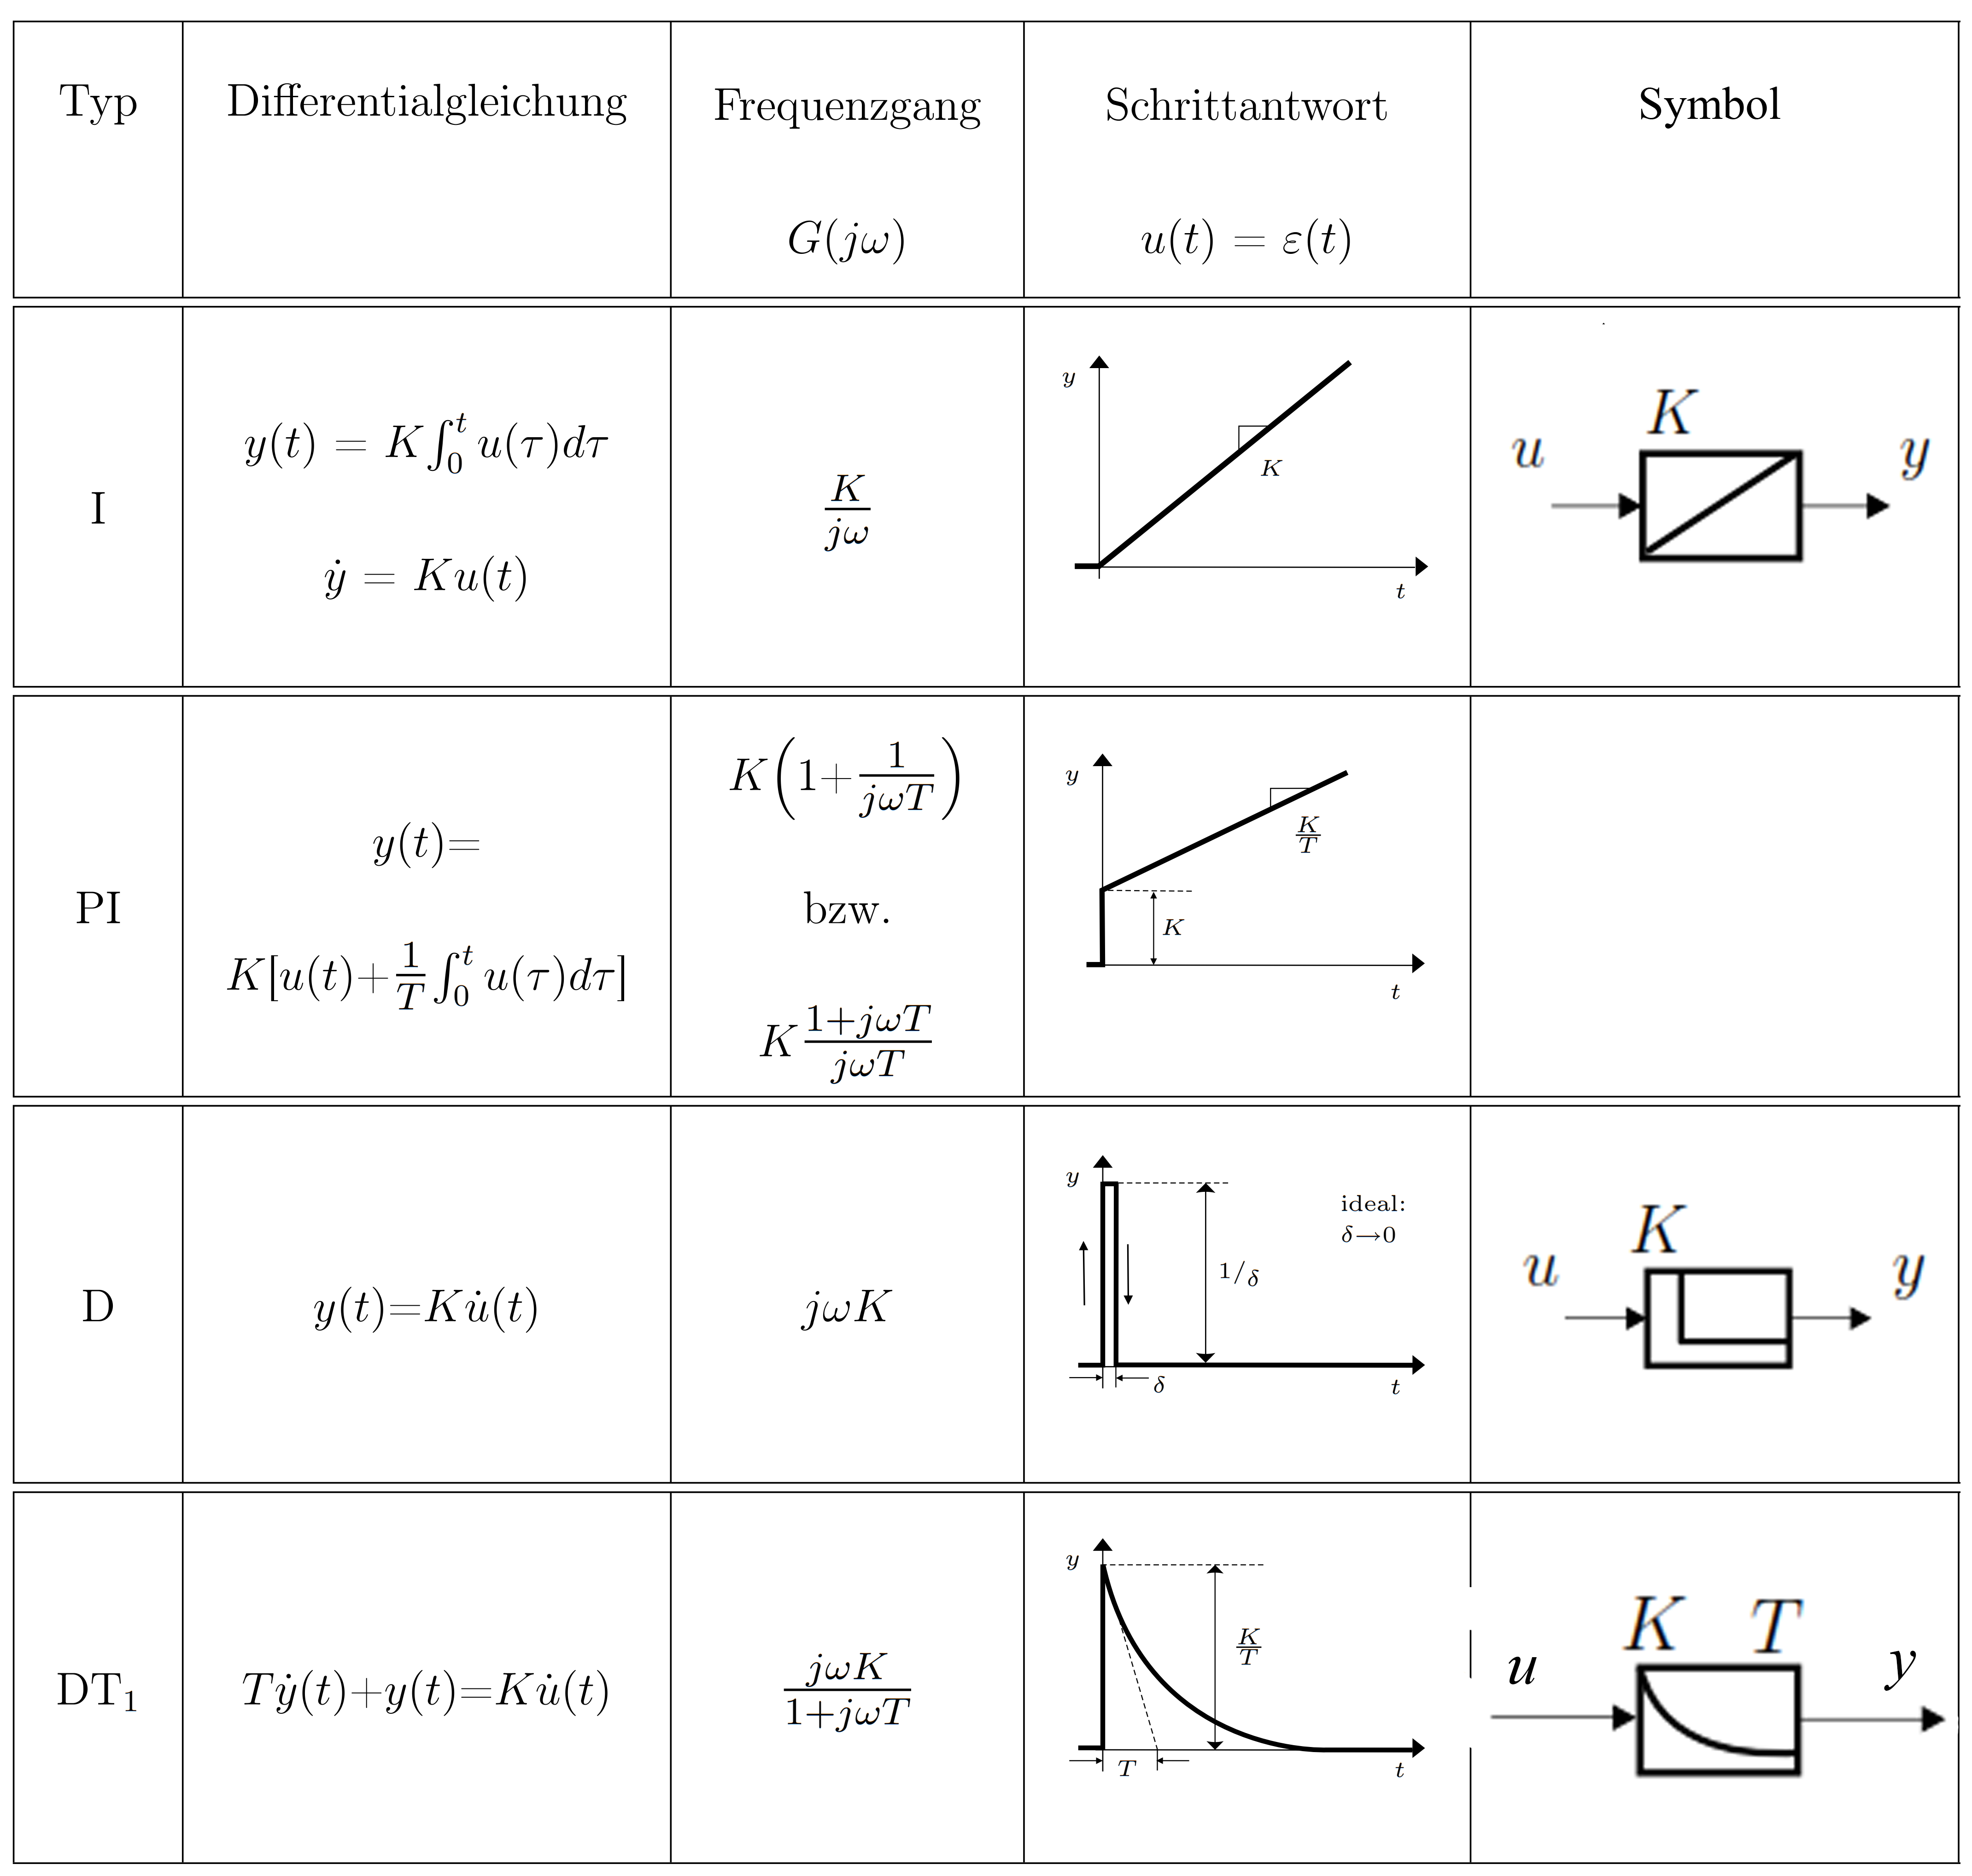
\includegraphics[width=13.5 cm]{./bilder/grundglieder/tabelle/glieder3.png} \\
			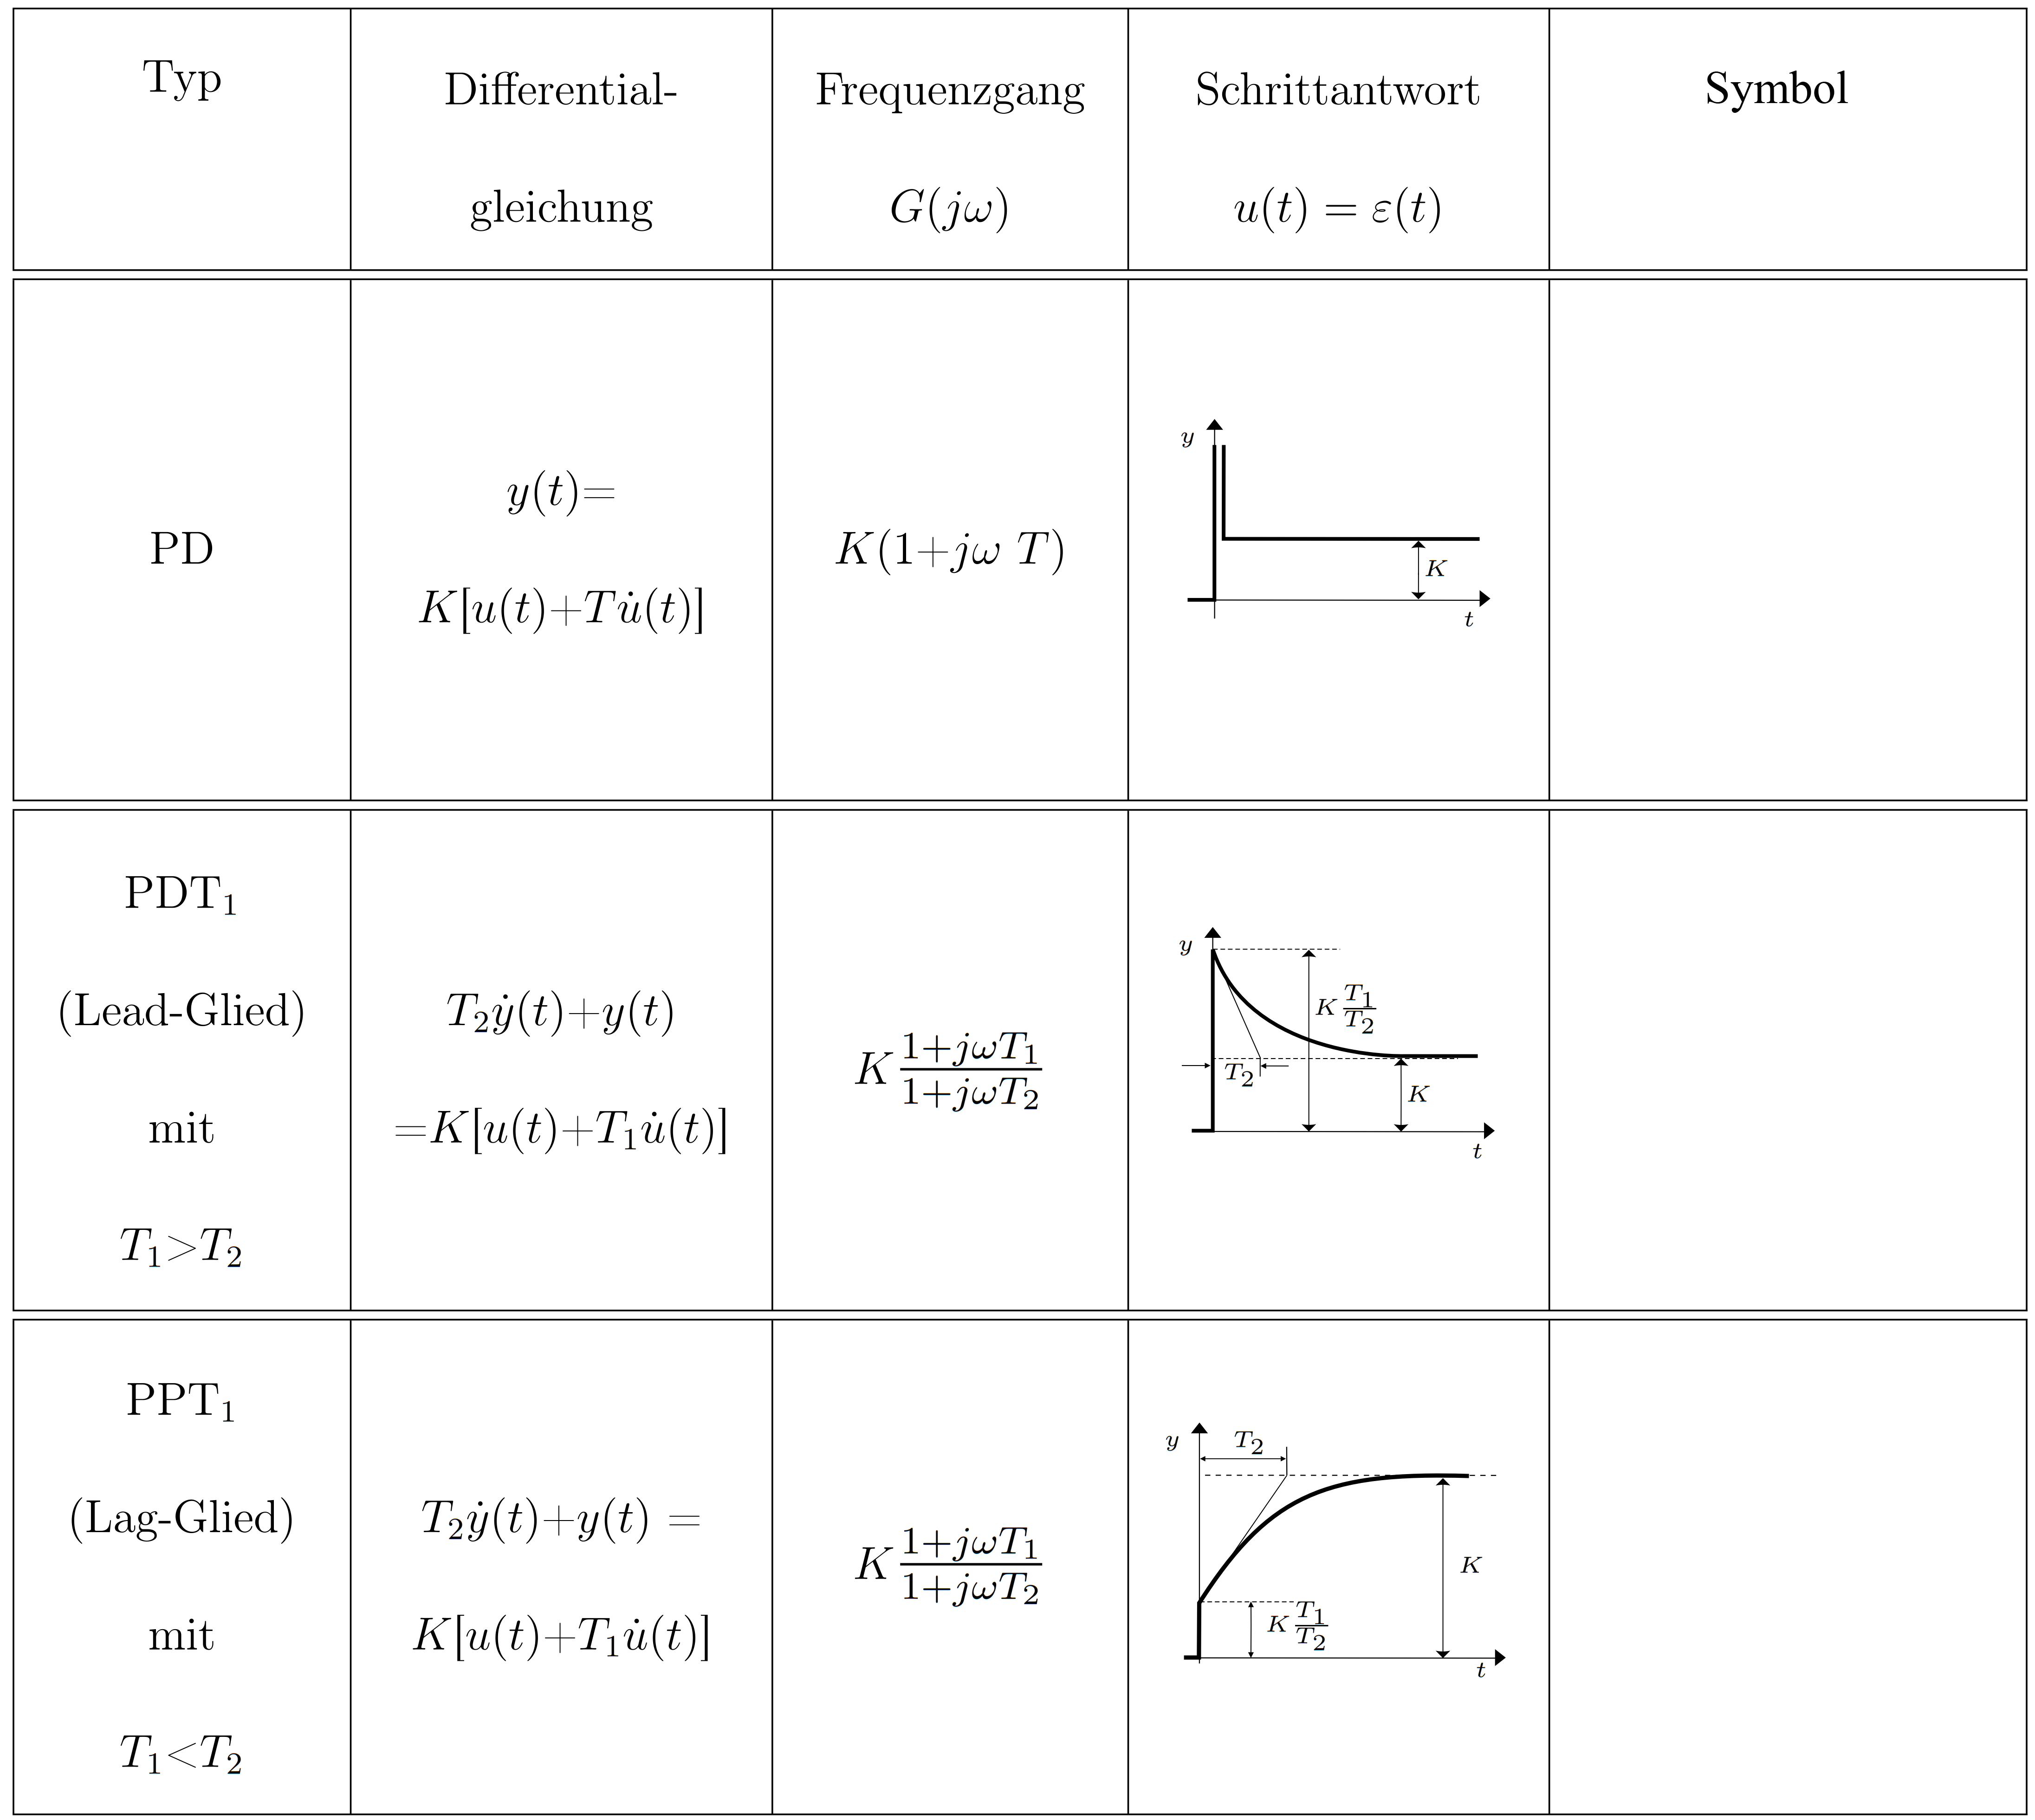
\includegraphics[width=13.5 cm]{./bilder/grundglieder/tabelle/glieder4.png} \\
			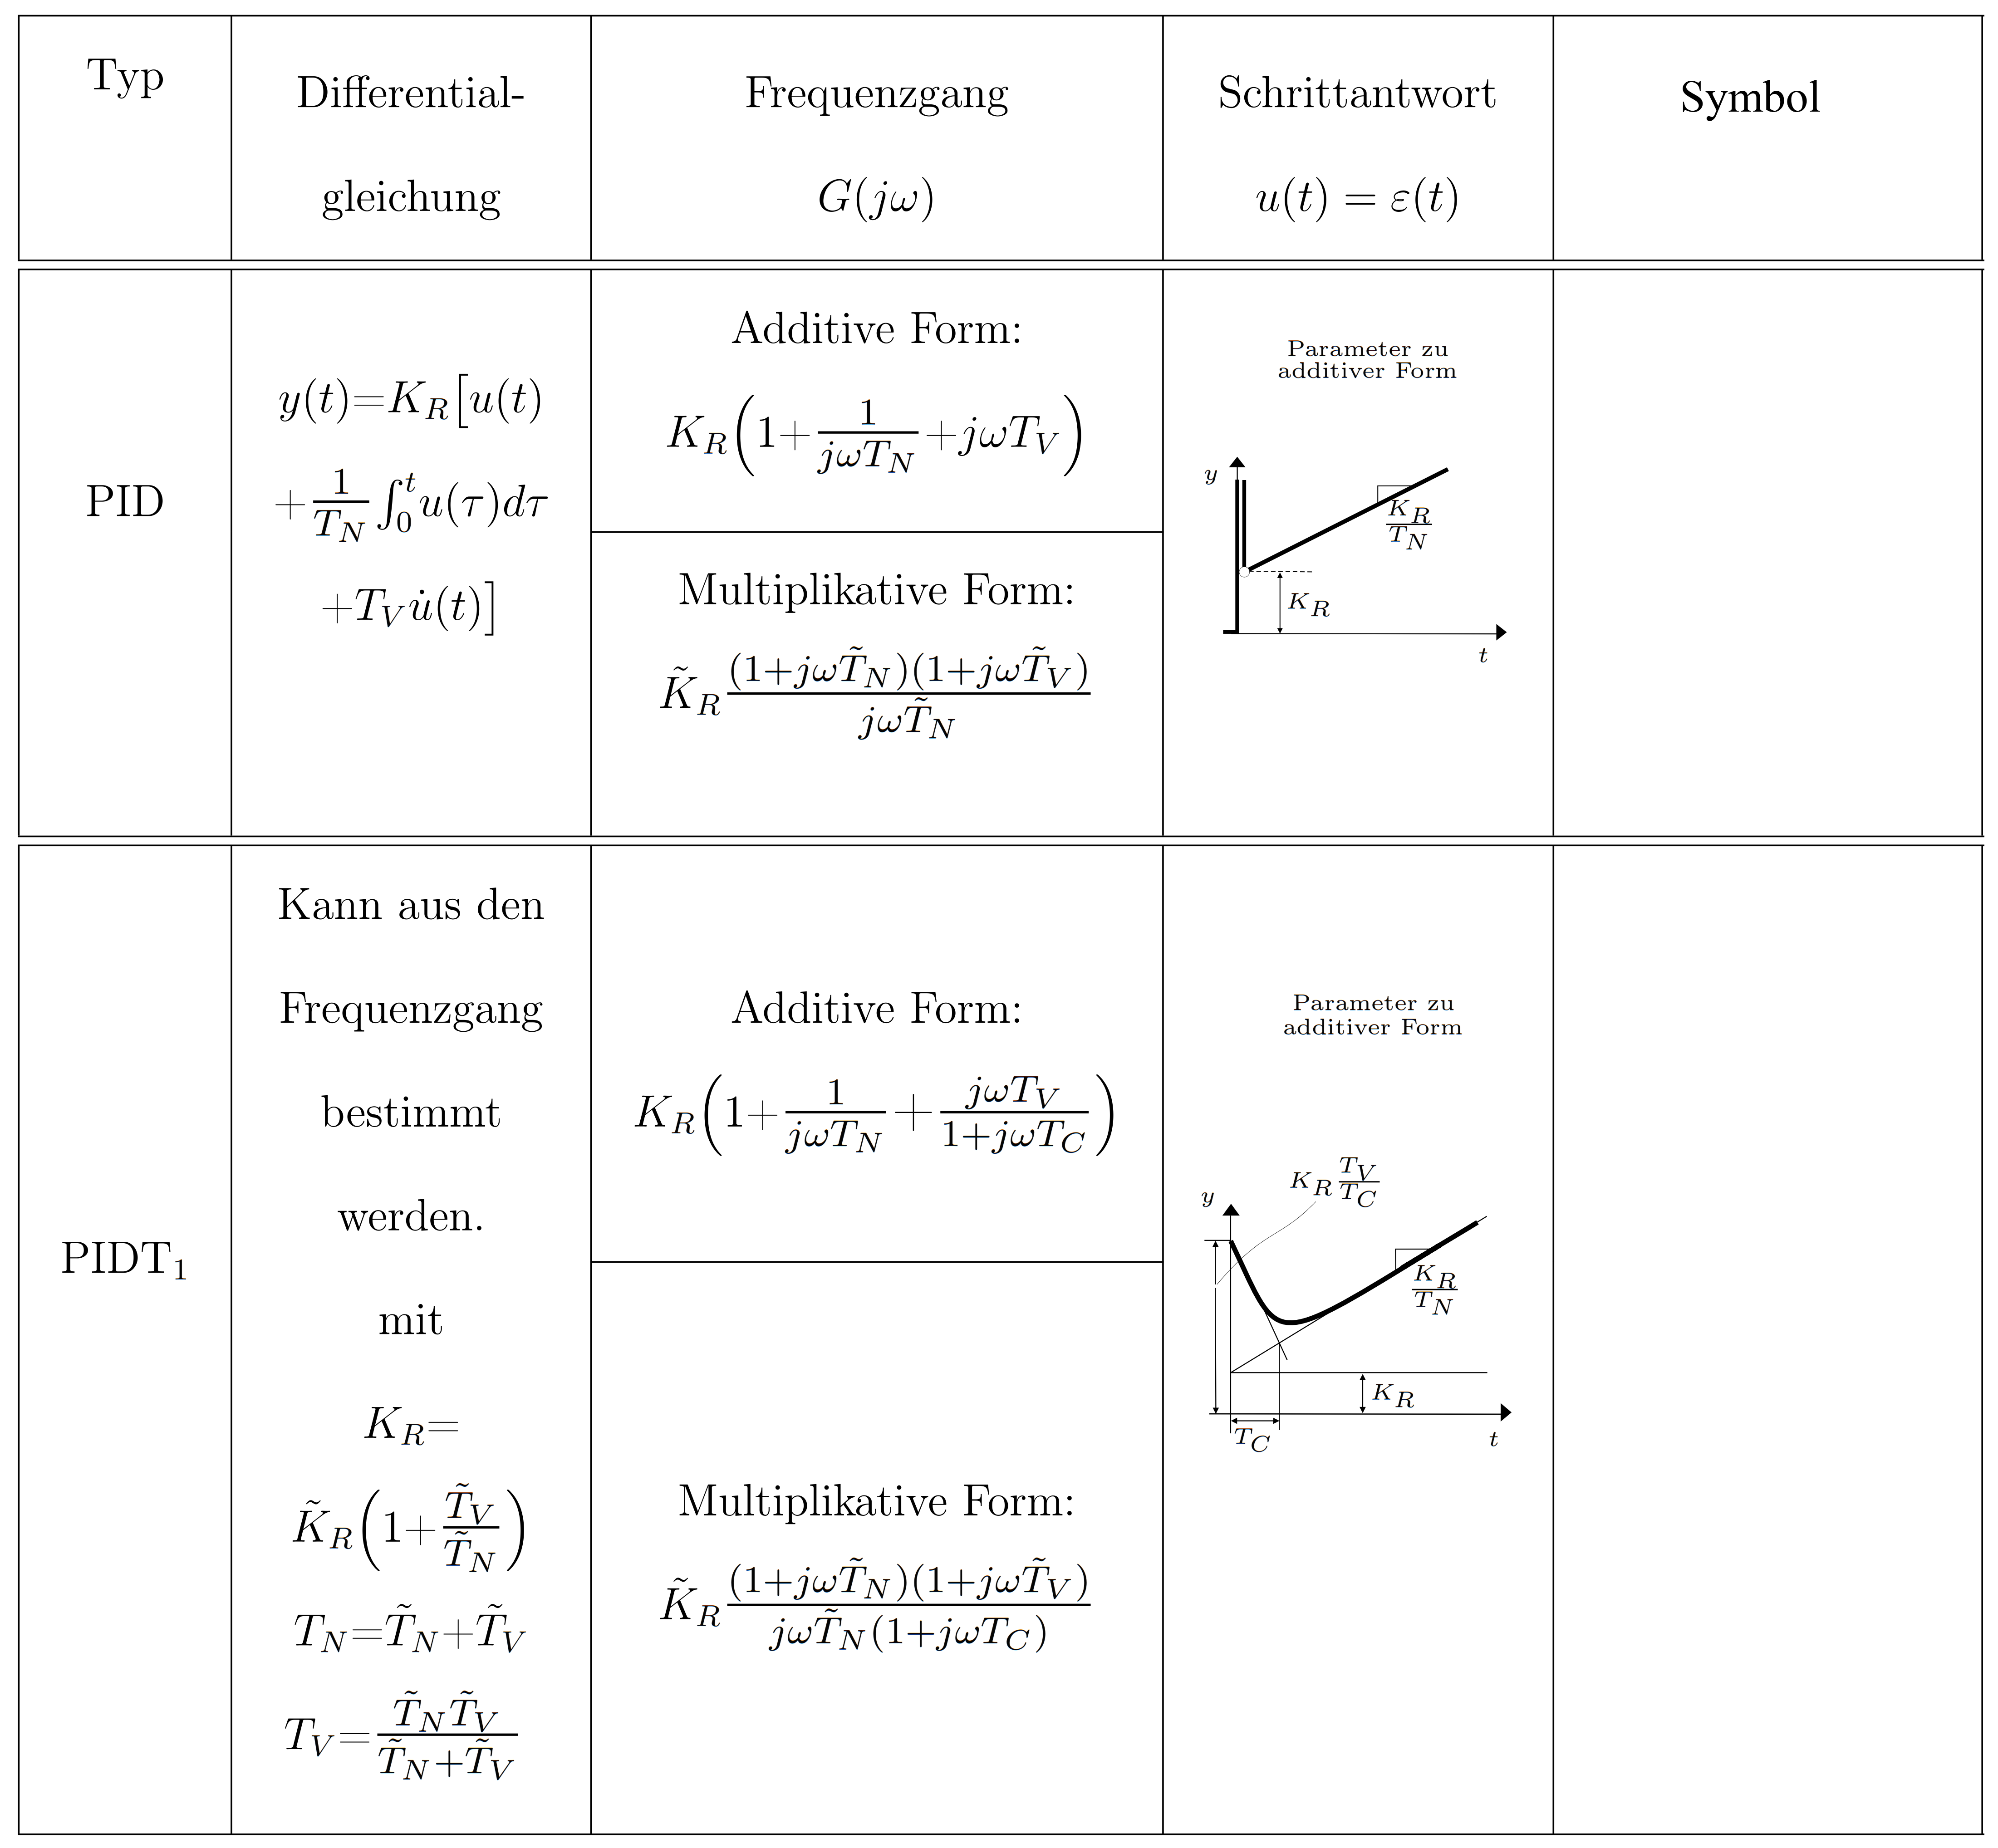
\includegraphics[width=13.5 cm]{./bilder/grundglieder/tabelle/glieder5.png} \\
			
	\subsection{LZI-Systeme, vertauschen von Blöcken \skript{81}}
		$\Rightarrow$ \quad aus Platzgründen siehe: Skript S. 81
			
%TODO Kap. Grundglieder: mit Beispiele neben Tabelle aus Buch Regelungstechnik für Ingenieure ab S. 487; Bilder ausschneiden und mit Minipages pro Zeile arbeiten
%			\begin{tabular}{l|l}
%					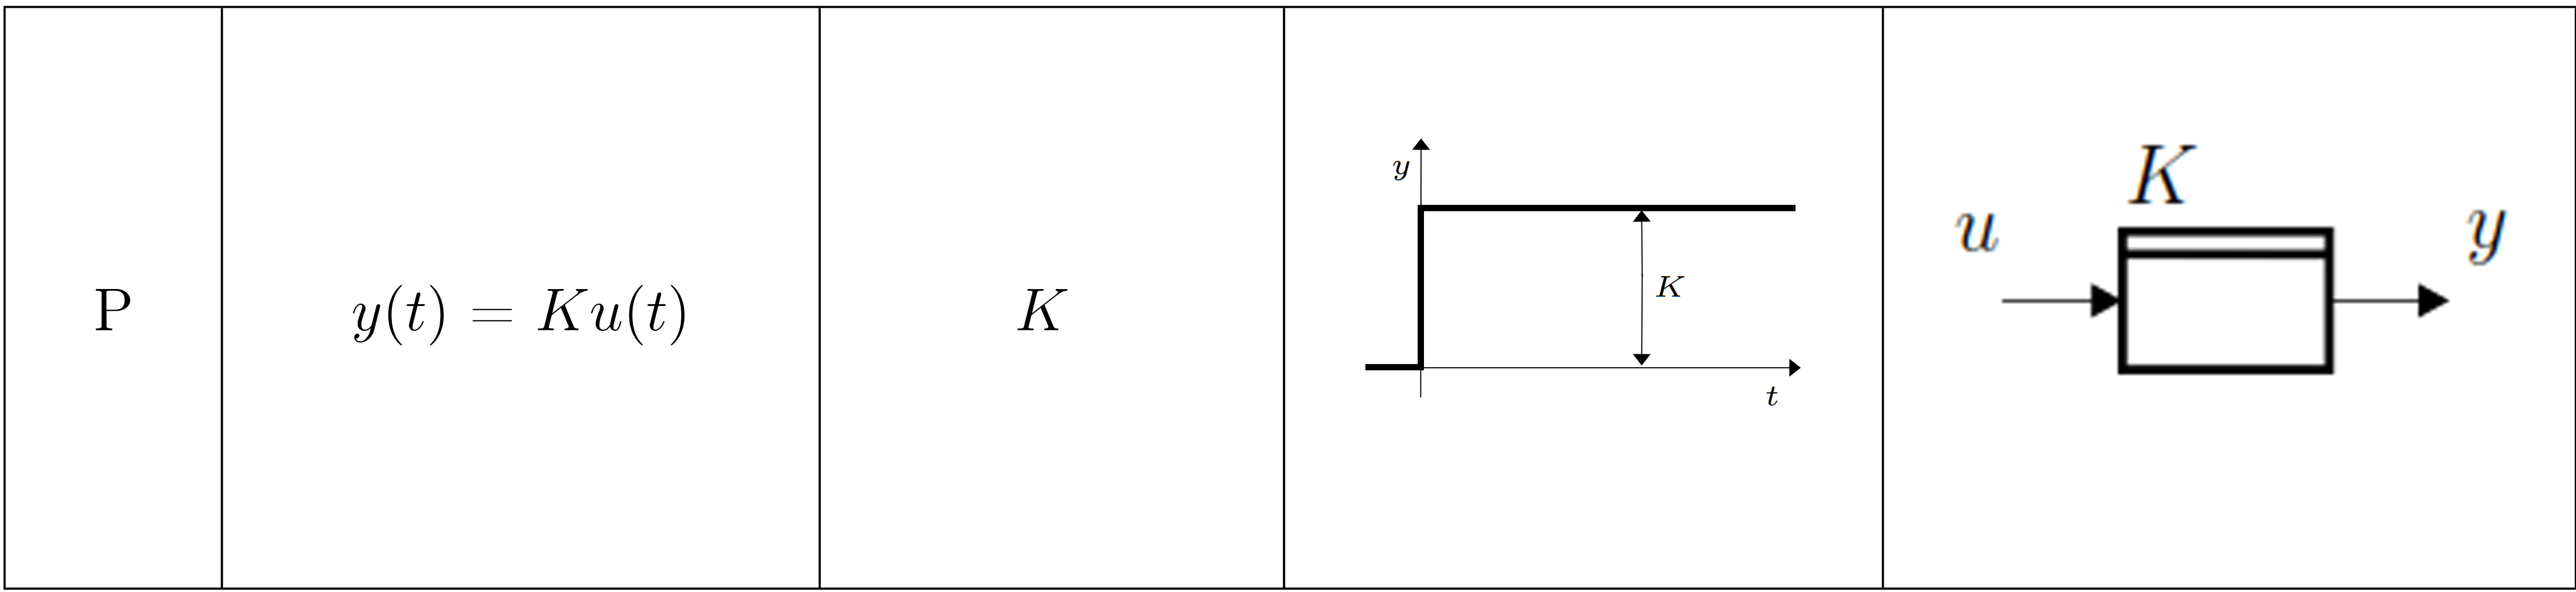
\includegraphics[width=13.5 cm]{./bilder/grundglieder/einzeln/pGlied.png}	&  \\
%				\hline
%					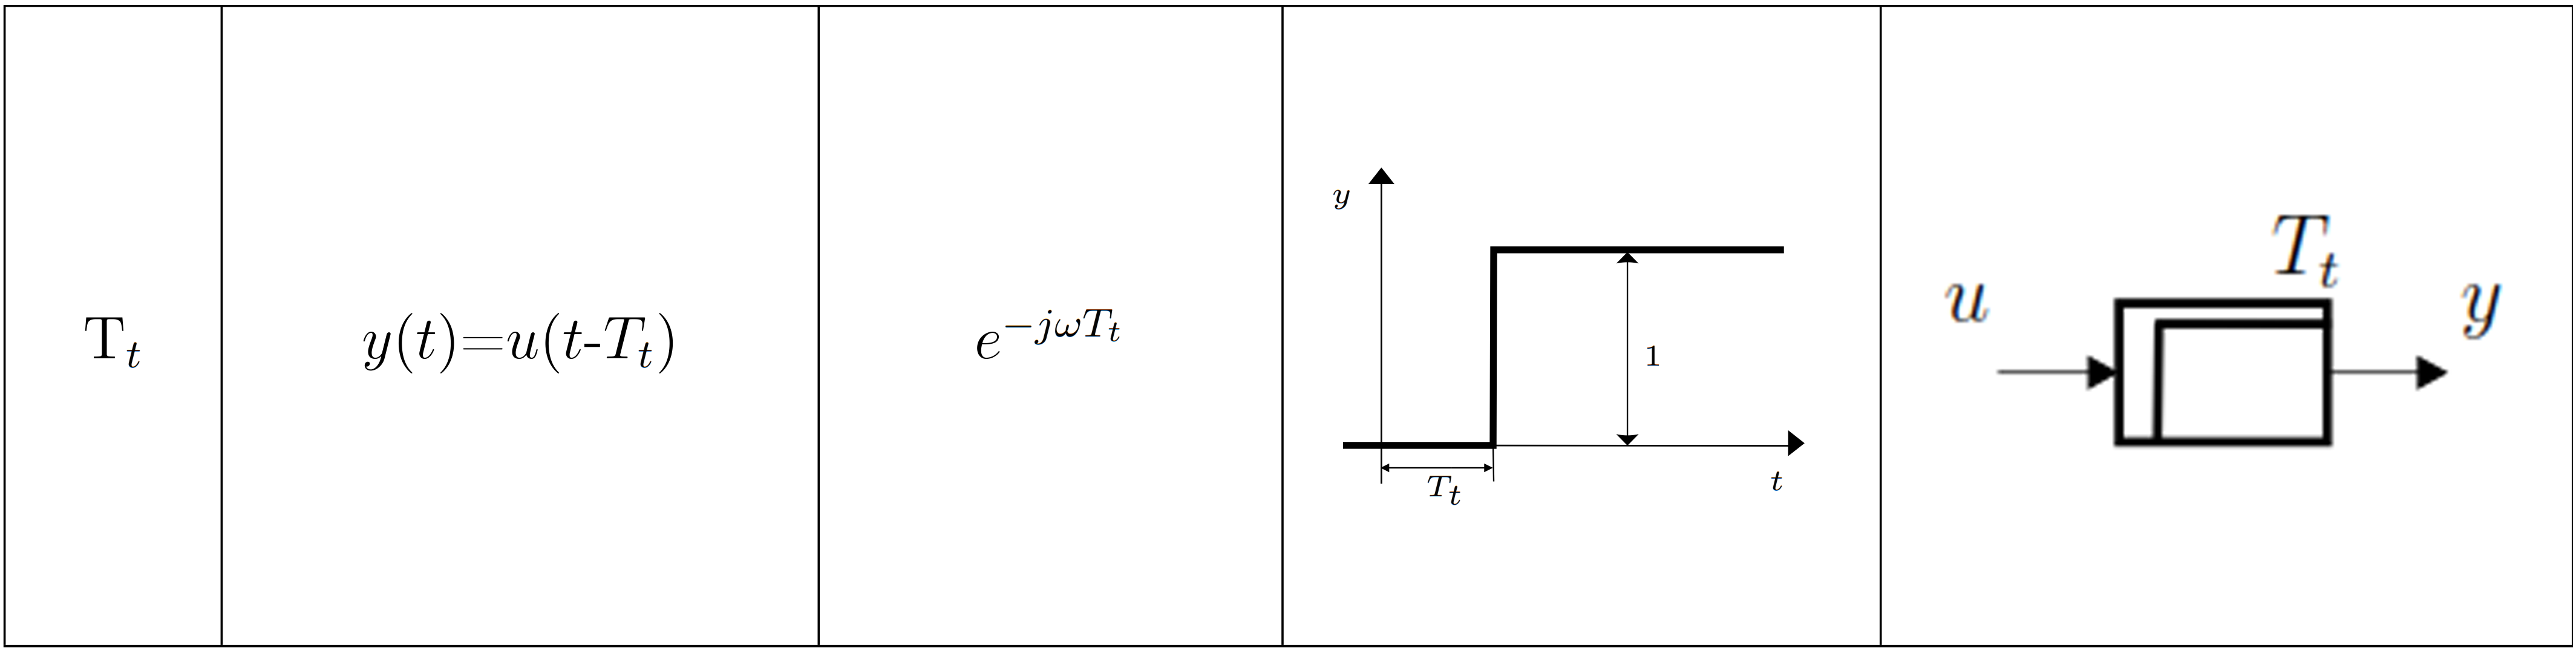
\includegraphics[width=13.5 cm]{./bilder/grundglieder/einzeln/tGlied.png}	&  \\
%				\hline
%					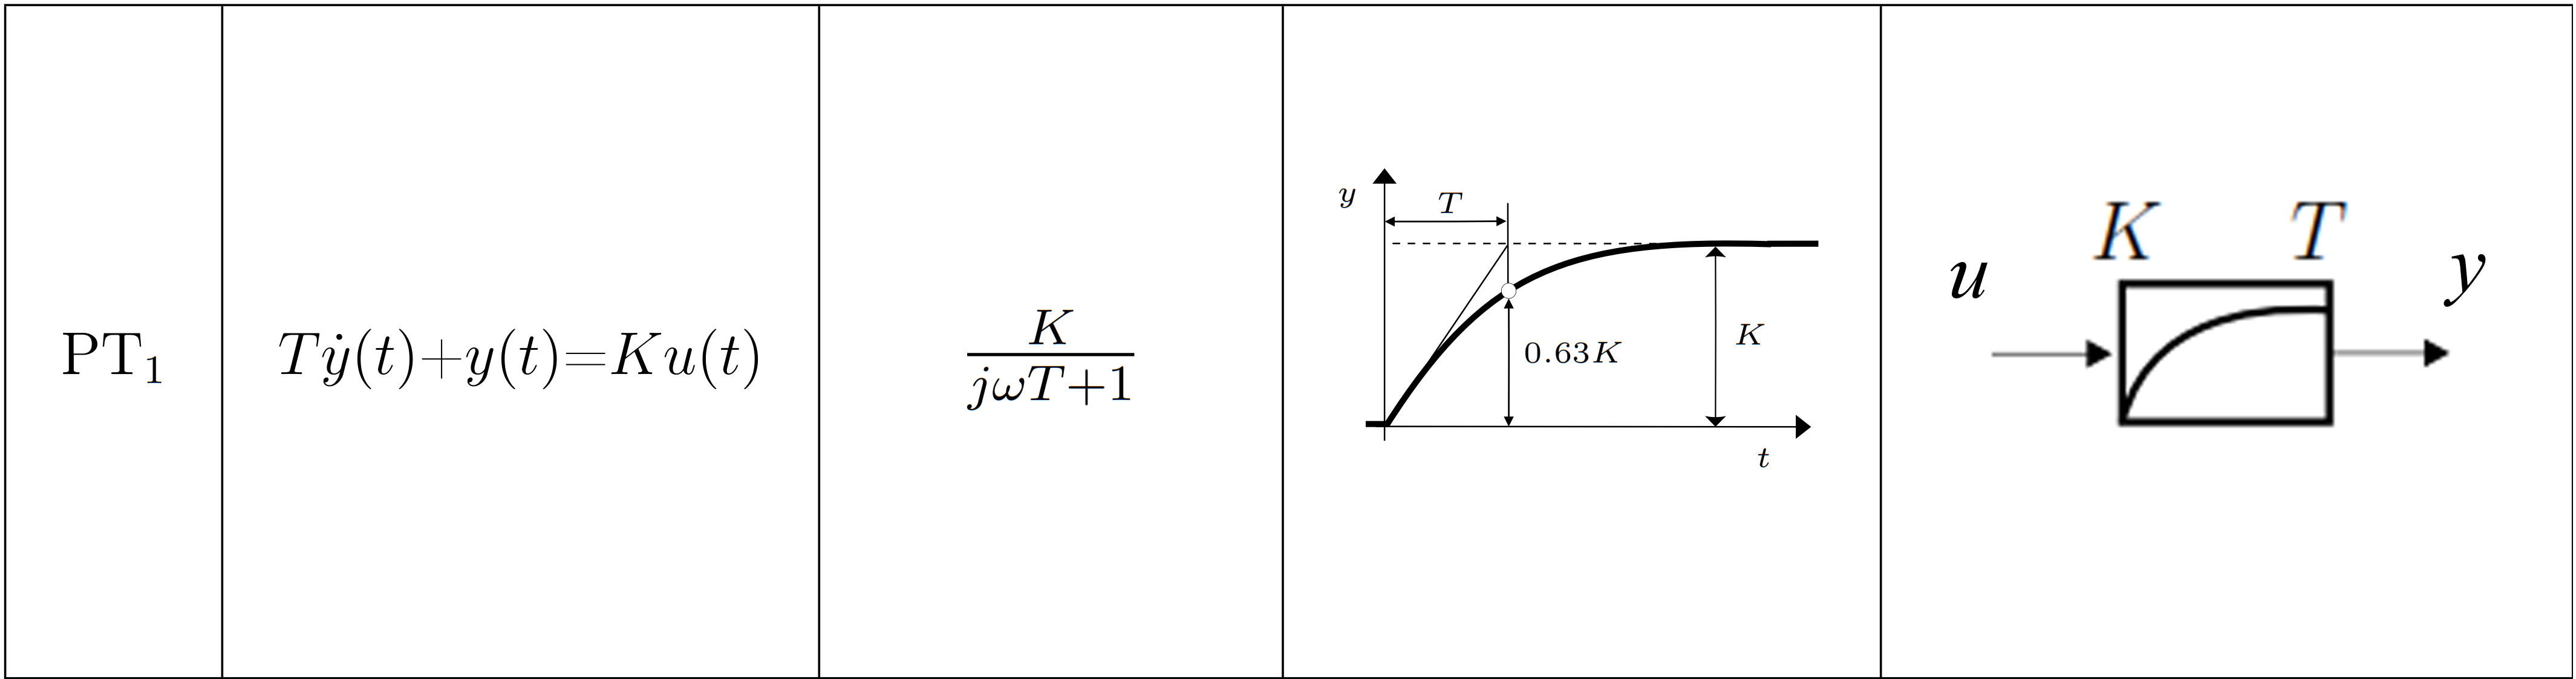
\includegraphics[width=13.5 cm]{./bilder/grundglieder/einzeln/pt1Glied.png}	&  \\
%				\hline
%			\end{tabular}
%		
%			\begin{tabular}{l|l}
%					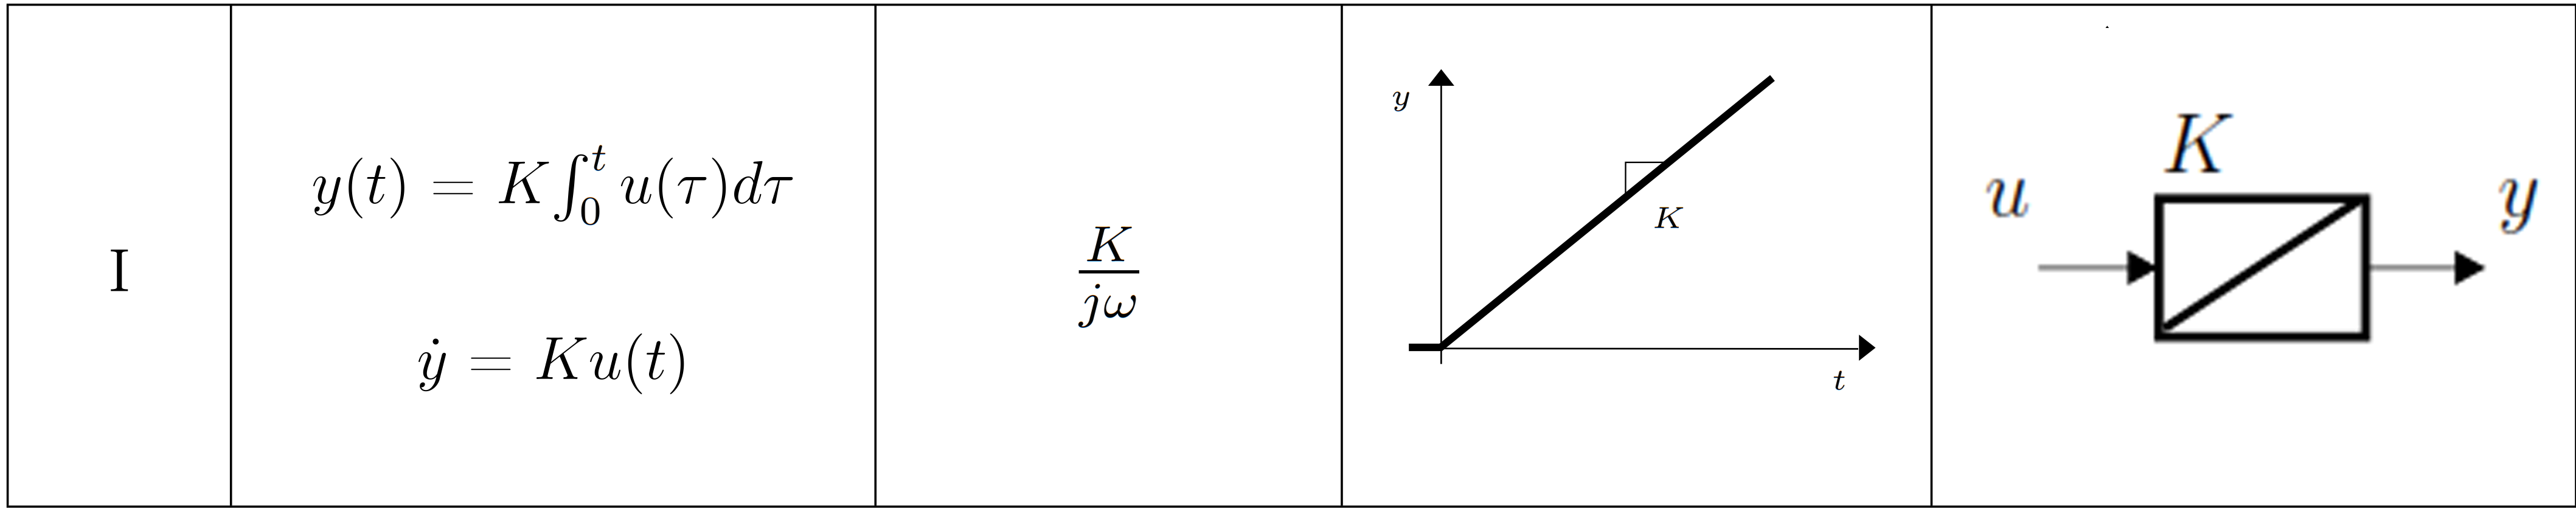
\includegraphics[width=13.5 cm]{./bilder/grundglieder/einzeln/iGlied.png}	&  \\
%				\hline
%					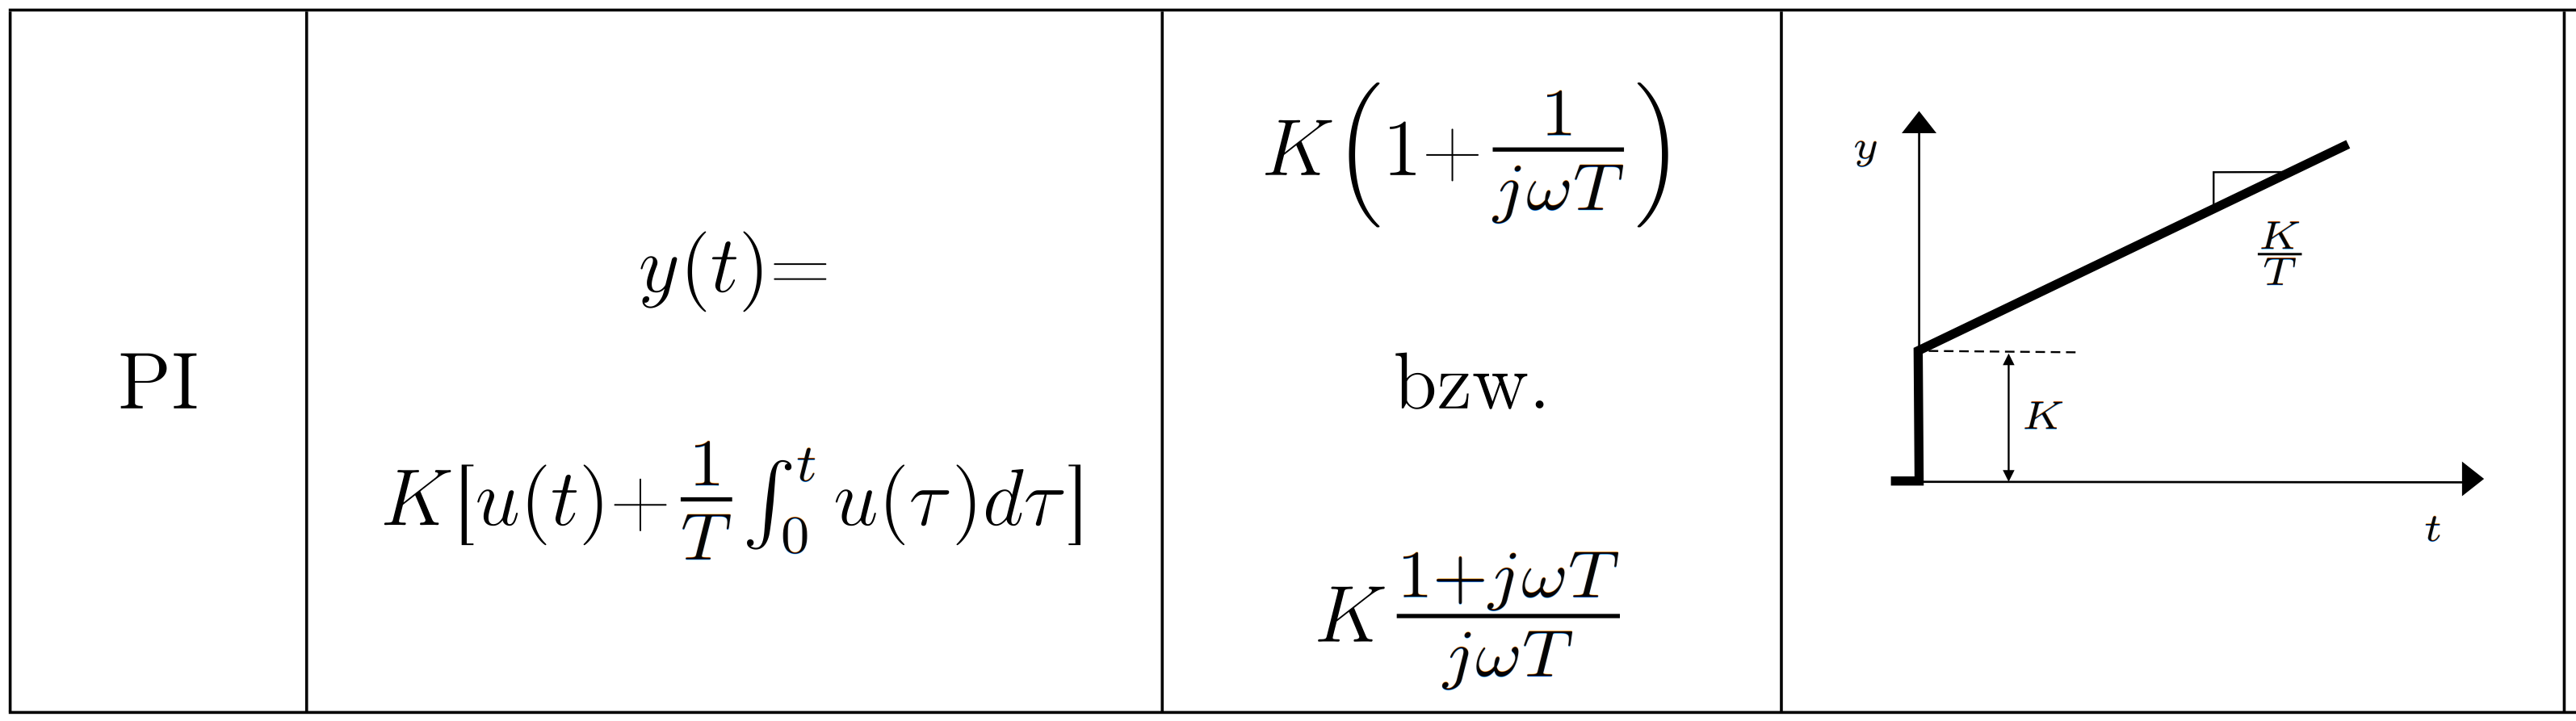
\includegraphics[width=13.5 cm]{./bilder/grundglieder/einzeln/piGlied.png}	&  \\
%				\hline
%					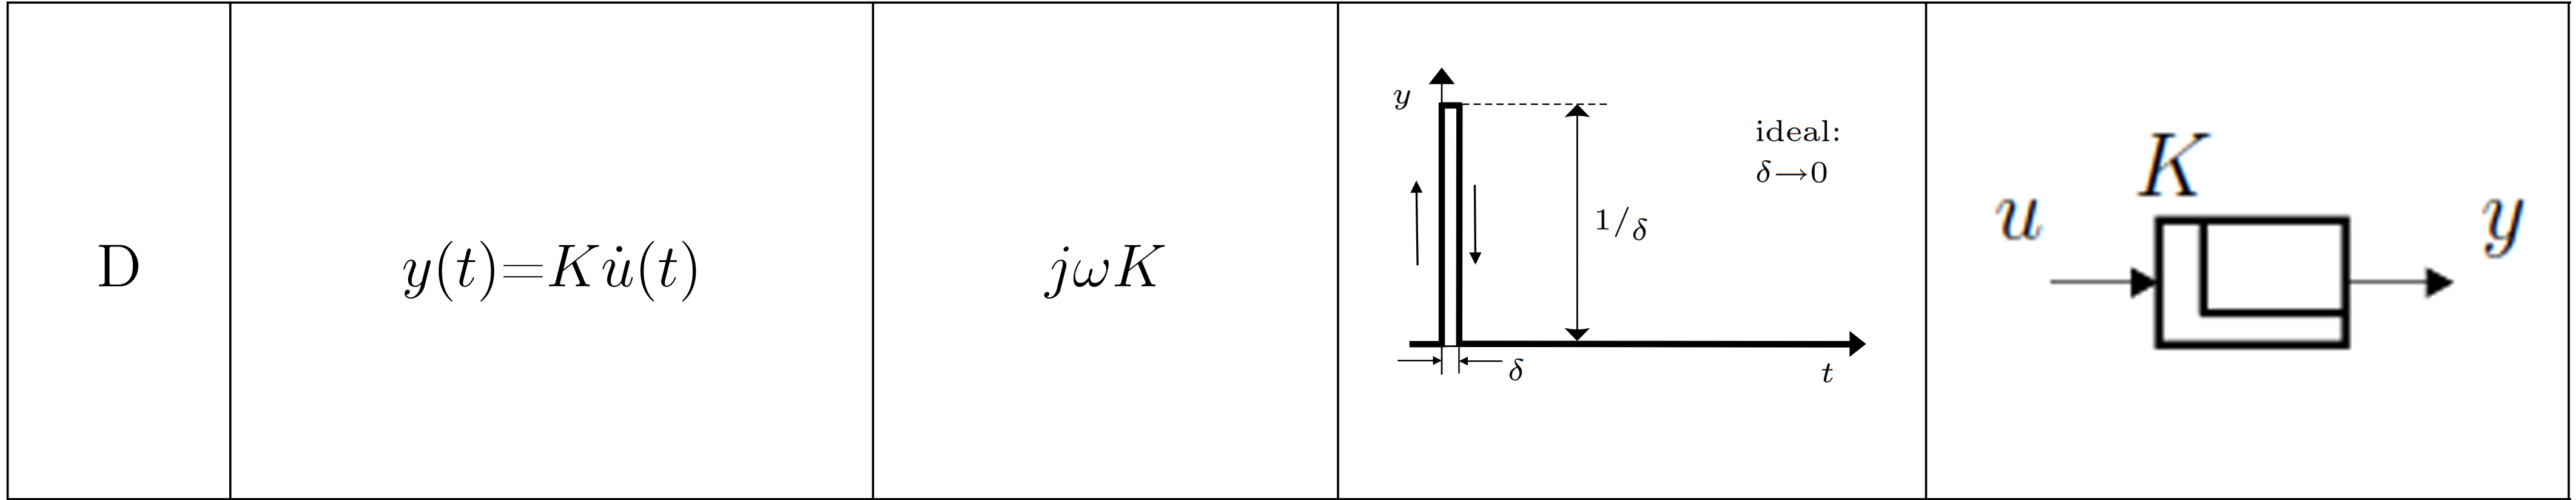
\includegraphics[width=13.5 cm]{./bilder/grundglieder/einzeln/dGlied.png}	&  \\
%				\hline
%					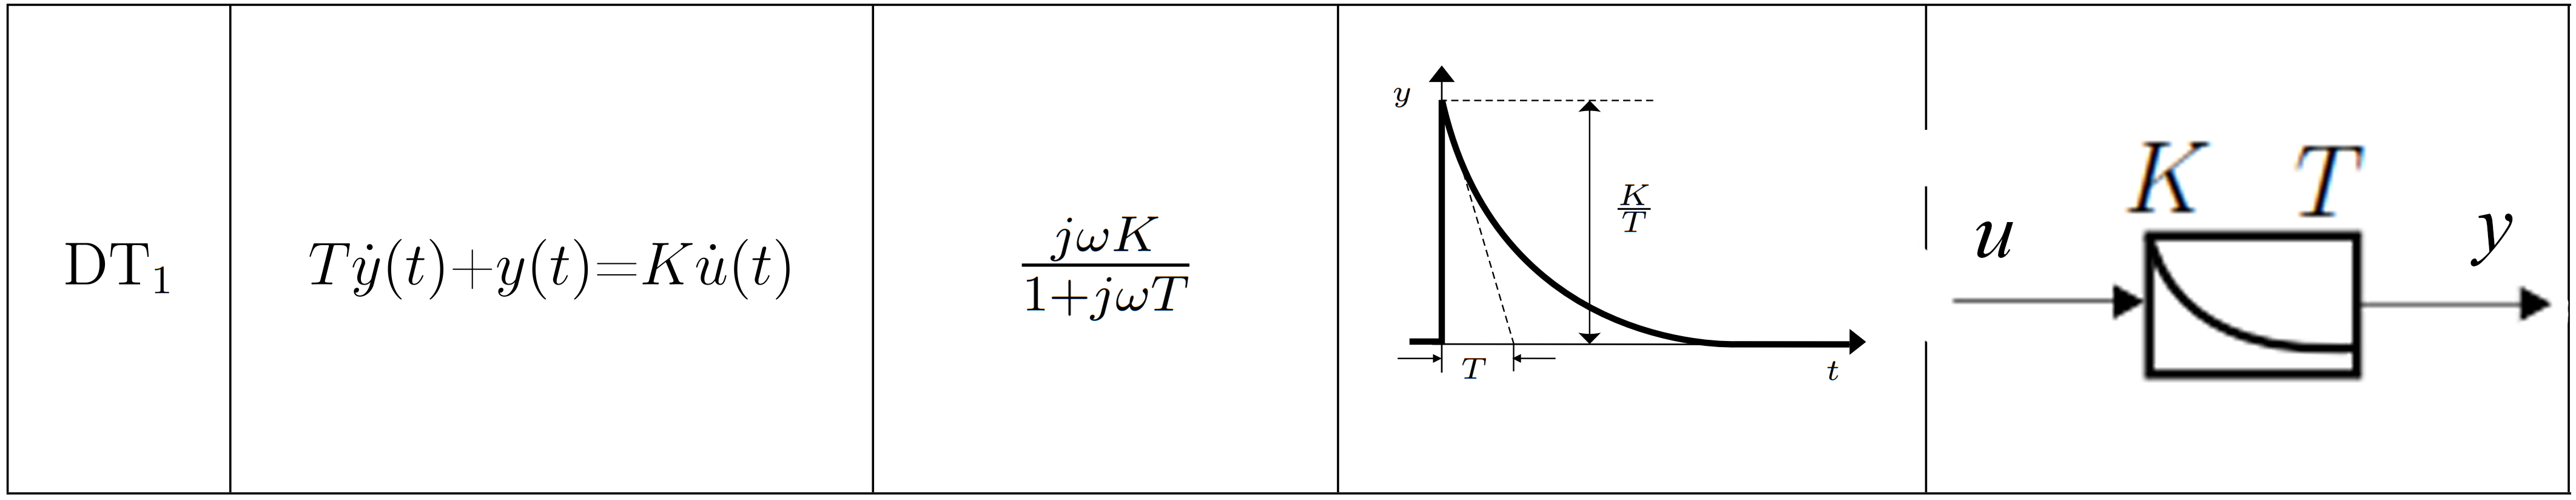
\includegraphics[width=13.5 cm]{./bilder/grundglieder/einzeln/dt1Glied.png}		& \\
%				\hline
%			\end{tabular}




